%%
%%
\documentclass[12pt]{book}
\usepackage{amsfonts}
\usepackage{amsmath}
\usepackage{amssymb}
\usepackage{graphicx}
\usepackage{hyperref}
\usepackage{tabularx}
\usepackage{float}
\setlength{\textheight}{10in}
\setlength{\textwidth}{7.4in}
\setlength{\topmargin}{-0.75in}
\setlength{\oddsidemargin}{-0.5in}
\setlength{\evensidemargin}{-0.5in}
\setlength{\parskip}{0.15in}
\setlength{\parindent}{0in}

\begin{document}


\vspace{-1.0in}\begin{center}
\Large{MHF4UR : Pre-AP Advanced Functions }

\Large{Assignment \#2}


\end{center}

%\medskip

\vspace{0.015in}\hrulefill\ 

\textbf{Reference Declaration} %  Fill in your Reference Declarations in this section before your submit your assignment.

Complete the Reference Declaration section below in order for your assigment to be graded.

If you used any references beyond the course text and lectures (such as other texts, discussions with colleagues or online resources), indicate this information in the space below.  If you did not use any aids, state this in the space provided. 

Be sure to cite appropriate theorems throughout your work. You may use shorthand for well-known theorems like the FT (Factor Theorem), RRT (Rational Root Theorem), etc. 

Note: Your submitted work must be \textbf{your original work}. 

Family Name: Do\\%Family Name Here
First Name: Kien%First Name Here

Declared References: Used the website below to review Partial Fraction Decomposition for question 4.\\ https://www.purplemath.com/modules/partfrac.htm\\
Asked my dad to teach me induction as well as used the website below for the proof by induction question.\\
https://www.mathsisfun.com/algebra/mathematical-induction.html\\

% Type your references here.
% You can use as many lines as required.

\vspace{0.015in}\hrulefill\ 

\newpage

%%%%%%%%%%%% PROBLEMS START HERE

\begin{enumerate}

%% PROBLEM 1
\item Solve $\dfrac{x^{9000}+9001}{x^{9002}+9003} \le 0$\\

Firstly, let's take a look at the denominator of this inequality.\\

\textbf{Proof that the denominator of the function is positive.}\\\\
We can see that $x^{9002}+9003$ is a polynomial function with an even degree, therefore, this function will have characteristics of an even degree function. One of the characteristics that this function must have is that it has like end behaviours. Since the leading coefficient is +1 and the term with the highest degree is the the only term that contains the variable $x$, this function opens up. In addition, this function is also vertically translated 9003 units up.\\
These facts prove that the denominator yields only positive values, therefore, multiplying both sides by the denominator without changing the inequality sign is a valid action since we are multiplying by a positive number.\\
\begingroup
\addtolength{\jot}{1em}
\begin{align}
    \dfrac{x^{9000}+9001}{x^{9002}+9003} \times (x^{9002}+9003) &\le 0 \times (x^{9002}+9003)\\
    x^{9000}+9001 &\le 0z
\end{align}
\endgroup

For the function on line (2) above, there is no real value for $x$ such that the output is $\leq 0$ because $x^{9000}+9001$ can never be less than or equal to 0.\\

Explanation: $x^{9000}+9001$ is an even function which means it has like end behaviours. Since $X^{9000}$ is the only term that is not a constant, the function opens up like a quadratic equation, therefore it has a greatest lower bound. Since the function is translated 9001 units up, its greatest lower bound or minimum value is 9001.\\

\textbf{Therefore, there exists no real value for $x$ to satisfy this inequality.}

\newpage

%% PROBLEM 2
\item Determine the equation of a rational function which has all of the characteristics below or explain and prove why it cannot exist: 

\begin{enumerate}
\item 4 vertical asymptotes\\

For a rational function to have a vertical asymptote(s), the denominator must contain the input variable $x$.\\
1. The number of vertical asymptotes can be determined by the largest exponent in the denominator provided that the denominator be a polynomial function in factored form where each factor has a different zero and is of multiplicity 1.\\
2. Where the vertical asymptotes are located at can be determined by the zeros of the functions written in factored form.\\

For this characteristic, the highest degree of the denominator must be at least 4 for there to be 4 vertical asymptotes.

\item 2 point discontinuities\\

For there to be 2 point discontinuities, two restrictions on the $x$-axis/domain will work, provided that the restriction does not have the same value on the $x$-axis as the 4 vertical asymptotes.

\item is negative on exactly 2 intervals\\

Since the function is divided into 5 parts (it has 4 vertical asymptotes), as long as 2 parts and only 2 parts output values that are less than 0, this characteristic will be satisfied.\\

However, another case where this characteristic will be true is when 1 part outputs a parabola or a parabola-like function that is reflected on the x-axis with its maximum value be equal to 0 - the rest of the function will output values larger or equal to 0.\\

So, either one of the five divided parts of the function outputs values less than AND equal to 0, or two of the five divided parts that outputs values less than 0 but not equal to 0.

\item has 5 zeros\\

To make it easier to determine a rational function that works with this characteristic, the function can be in factored form as follows:
$$a * b * c * d * e$$
where $a, b, c, d, e$ are in the form $\dfrac{(x+a)^n}{(x+b)^m} \quad (a,b \in \mathbb{R}, n,m \in \mathbb{N}$ including 0)

\item is even\\

For the function to be even, $f(x)$ has to equal $f(-x)$. For $f(x)$ to equal $f(x)$, the highest degree of the entire rational function must be of even degree.
\end{enumerate}
\newpage

\textbf{Conclusion:} After closely examining all of the characteristics and seeing if the characteristics comply with each other or not, I've come to a conclusion that there does exist a rational function that has all of the characteristics. The final graph the complies with all characteristics is:
\begin{figure}[H]
\centering{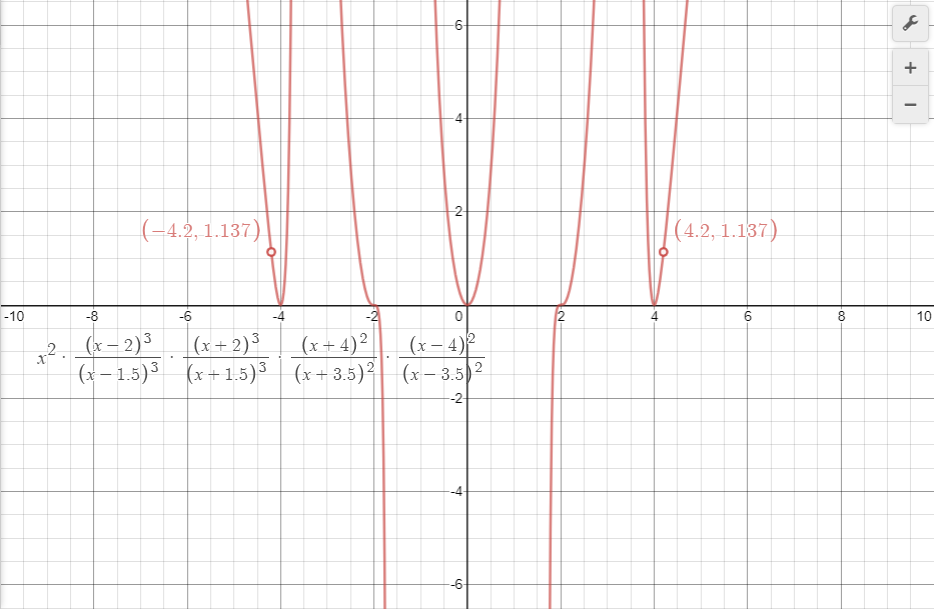
\includegraphics[width=15cm]{Q2Final.png}}
\caption{Final graph}
\end{figure} 

\textbf{Therefore, a rational function that complies with all of 5 characteristics does exist.}

\newpage

%% PROBLEM 3
\item Solve $\dfrac{7}{x+2} + \dfrac{5}{x-2} = \dfrac{10x-2}{x^2 - 4}$.\\

\textbf{Solution:}

\begingroup
\addtolength{\jot}{1em}
\begin{align*}
    \dfrac{7}{x+2} + \dfrac{5}{x-2} &= \dfrac{10x-2}{x^2 - 4}\\
    \dfrac{7(x-2) + 5(x+2)}{(x+2)(x-2)} &= \dfrac{10x-2}{(x+2)(x-2)}\\
    7x-14+5x+10 &= 10x - 2\qquad\qquad\qquad\quad(x \neq 2, -2)\\
    12x-4-(10x-2) &= 0\qquad\qquad\qquad\qquad\qquad(x \neq 2, -2)\\
    2x-2 &= 0\qquad\qquad\qquad\qquad\qquad(x \neq 2, -2)\\
    x &= 1\qquad\qquad\qquad\qquad\qquad(x \neq 2, -2)
\end{align*}
\endgroup
\textbf{Therefore x = 1.}

\newpage

%% PROBLEM 4
\item Determine values $A,B,C, \in \mathbb{R}$ such that $\dfrac{2x+1}{x^3-x} = \dfrac{A}{x}+\dfrac{B}{x+1}+\dfrac{C}{x-1}$ is an identity.\\

\textbf{Solution:}\\
Step 1: Decompose the denominator on the left side to make it equal the right side. Add the right side.
\begingroup
\addtolength{\jot}{1em}
\begin{align*}
    \dfrac{2x+1}{x^3 - x} &= \dfrac{A}{x}+\dfrac{B}{x+1}+\dfrac{C}{x-1}\\
    \dfrac{2x+1}{x(x^2-1)} &= \dfrac{A(x+1)(x-1) + Bx(x-1) + Cx(x+1)}{x(x-1)(x+1)}\\
    \dfrac{2x+1}{x(x-1)(x+1)} &= \dfrac{Ax^2 - A + Bx^2 - Bx + Cx^2 + Cx}{x(x-1)(x+1)}\\
    \dfrac{2x+1}{x(x-1)(x+1)} &= \dfrac{x^2(A+B+C) + x(C-B) - A}{x(x-1)(x+1)}
\end{align*}
\endgroup

Step 2: Now, we can remove the denominator on both sides of the equation and declare restrictions.
\begin{align*}
    2x+1 &= x^2(A+B+C) + x(C-B) - A \qquad\qquad\qquad (x \neq 0, -1, 1)
\end{align*}
Step 3: Let $A+B+C = 0$, $C-B = 2$ and $-A = 1$ so that it is in the same form as $2x + 1$.
\begin{align*}
    2x+1 &= x^2(A+B+C) + x(C-B) - A \qquad\qquad\qquad (x \neq 0, -1, 1)\\
    2x+1 &= x^2 \times (0) + x \times (2) + 1 \qquad\qquad\qquad\qquad\qquad (x \neq 0, -1, 1)
\end{align*}
Step 4: Determine $A$, $B$ and $C$.\\
We now have the following:
\setcounter{equation}{0}
\begin{align}
    A+B+C &= 0\\
    C - B &= 2\\
    A &= -1
\end{align}
Sub $A = -1$ into line (1).
\begin{align}
    -1+B+C &= 0\\
    B+C&= 1
\end{align}
Determine $C$ using elimination.
\begin{align}
    B+C = 1&\\
    +\quad-B + C = 2&\\
    \rule{4cm}{0.4pt}&\\
    2C = 3&\\
    C = \dfrac{3}{2}&
\end{align}
Determine $B$ by subbing in $C = \dfrac{3}{2}$ into line (7).
\begin{align}
    -B + 1&= 2\\
    B &= C - 2\\
    B &= \dfrac{3}{2} - \dfrac{4}{2}\\
    B &= -\dfrac{1}{2}
\end{align}
\textbf{Therefore, $A = -1$, $B = -\dfrac{1}{2}$, $C = \dfrac{3}{2}$.}

\newpage

%% PROBLEM 5
\item Solve $\bigg|\dfrac{x-4}{x+5}\bigg| \le 4$.\\

\textbf{Solution:}\\
First, let's look at the cases where $\bigg|\dfrac{x-4}{x+5}\bigg| = 4$.\\\\
For this equation to be true: $x$ cannot be -5 because the function would be undefined and the value before the absolute operation must either be 4 or -4. Let's examine both cases.\\
\begin{minipage}{.5\textwidth}
    \begin{align*}
    \textbf{Case 1a}\\
        \dfrac{x-4}{x+5} &= 4 \\
        x-4 &= 4x + 20 \\
        -3x &= 24 \\ 
        x &= -8
    \end{align*}      
    \end{minipage}
    \begin{minipage}{.5\textwidth}
    \begin{align*}
    \textbf{Case 1b}\\
        \dfrac{x-4}{x+5} &= -4 \\
        x-4 &= -4x - 20 \\
        5x &= -16 \\ 
        x &= -\dfrac{16}{5}
    \end{align*}
\end{minipage}\\\\
\textbf{Therefore, $x = -8$ and $x = -\dfrac{16}{5}$ are both valid cases.}\\\\
Now, let's examine $x$ when $\bigg|\dfrac{x-4}{x+5}\bigg| < 4$.\\\\
We will remove the absolute operation. This will result in the inequality having two cases, case 2a and 2b.\\
For case 2a, the output is positive and for the output to be positive, $x < -5$ or $x \geq 4$.\\
For case 2b, the output is negative and for the output to be negative, $-5 < x < 4$. Similar to the previous cases, $x \neq -5$ otherwise this inequality would be undefined. The table below shows when the fraction is positive and when it is negative. This help to determine all possible values of $x$ and whether the numerator or denominator is positive or negative.\\\\
\begin{tabularx}{0.8\textwidth} { 
  | >{\raggedright\arraybackslash}X 
  | >{\centering\arraybackslash}X 
  | >{\centering\arraybackslash}X 
  | >{\raggedleft\arraybackslash}X | }
 \hline
  & $(-\infty, -5)$ & $(-5, 4)$ & $(4, \infty)$ \\
 \hline
 $(x-4)$ & - & - & + \\
 \hline
 $(x+5)$ & - & + & + \\
 \hline
 $f(x)$ & + & - & + \\
 \hline
\end{tabularx}\\\\

Simplify the two cases to make one side equal 0.
\newpage

\begingroup
\addtolength{\jot}{0.8em}
\begin{minipage}{.5\textwidth}
    \begin{align*}
    \textbf{Case 2a}\\
        \dfrac{x-4}{x+5} &< 4 \\
        \dfrac{x-4}{x+5} &< \dfrac{4(x+5)}{x+5} \\
        \dfrac{x-4}{x+5} - \dfrac{4(x+5)}{x+5} &< 0 \\
        \dfrac{x-4 - 4(x+5)}{x+5} \\
        \dfrac{x - 4 - 4x - 20}{x+5} &< 0 \\
        \dfrac{-3x-24}{x+5} &< 0 \\
        \dfrac{-3(x+8)}{x+5} &< 0 \\
        \dfrac{(x+8)}{x+5} &> 0 \\
    \end{align*}      
    \end{minipage}
    \begin{minipage}{.5\textwidth}
    \begin{align*}
    \textbf{Case 2b}\\
        \dfrac{x-4}{x+5} &> -4 \\
        \dfrac{x-4}{x+5} &> \dfrac{-4(x+5)}{x+5} \\
        \dfrac{x-4}{x+5}+\dfrac{4(x+5)}{x+5} &> 0 \\
        \dfrac{x-4+4(x+5)}{x+5} &> 0 \\
        \dfrac{x-4+4x+20}{x+5} &> 0 \\
        \dfrac{5x+16}{x+5} &> 0 \\
        \dfrac{5\left(x+\dfrac{16}{5}\right)}{x+5} &> 0 \\
    \end{align*}
\end{minipage}
\endgroup\\
To solve these two rational inequalities, draw out a factor table for each case.
\begin{center}
    \textbf{Case 2a}
\end{center}
\begin{tabularx}{0.8\textwidth} { 
  | >{\raggedright\arraybackslash}X 
  | >{\centering\arraybackslash}X 
  | >{\centering\arraybackslash}X 
  | >{\raggedleft\arraybackslash}X | }
 \hline
  & $(-\infty, -8)$ & $(-8, -5)$ & $(-5, \infty)$ \\
 \hline
 $(x+8)$ & - & + & + \\
 \hline
 $(x+5)$ & - & - & + \\
 \hline
 $f(x)$ & + & - & + \\
 \hline
\end{tabularx}\\\\
Since the output of this case is greater than 0, we will look at the values of the left column $x = (-\infty,-8)$ and the right column $(-5, \infty)$. These values must satisfy the conditions on the previous page where $x < -5$ and $x > 4$. We will take all values on the left column as it satisfies with the $x < -5$ condition, however, only part of the right column satisfies with $x > 4$. Therefore, we will ignore values from -5 to 4 and we will take all values from 4 to $\infty$, including 4.
%-----------   Case 2b   ----------------%
\begin{center}
    \textbf{Case 2b}
\end{center}
\begin{tabularx}{0.8\textwidth} { 
  | >{\raggedright\arraybackslash}X 
  | >{\centering\arraybackslash}X 
  | >{\centering\arraybackslash}X 
  | >{\raggedleft\arraybackslash}X | }
 \hline
  & $(-\infty, -5)$ & $\left(-5, -\dfrac{16}{5}\right)$ & $\left(-\dfrac{16}{5}, \infty\right)$ \\
 \hline
 $\left(x+\dfrac{16}{5}\right)$ & - &  - & +  \\
 \hline
 $(x+5)$ & -  & +  & +  \\
 \hline
 $f(x)$ &  +  & -  & +  \\
 \hline
\end{tabularx}\\\\
Since the output of this case is greater than 0, we will only look at the values on the left column $(-\infty, -5)$ and the right column, $\left(-\dfrac{16}{5}, \infty\right)$. Similar to case 2a, these values must also satisfy the condition on the previous page. In this case, the condition for $x$ is $-5 < x < 4$. The entire left column is less than -5 so we can safely ignore it. For the right column, we will only take the values from $\dfrac{-16}{5}$ to 4.

\textit{Conclusion:}\\
When all cases are gathered together and simplified, we have the following:\\

Case 1a and 1b: $x = -8, -\dfrac{16}{5}$\\\\
Case 2a: $x \in (-\infty, -8) \cup [4, \infty)$\\\\
Case 2b: $x \in \left(-\dfrac{16}{5}, 4\right)$

Combined answer: $x \in (-\infty, -8] \cup \left[-\dfrac{16}{5}, \infty\right)$\\

\textbf{Therefore:} $$x \in (-\infty, -8] \cup \left[-\dfrac{16}{5}, \infty\right)$$



\newpage

%% PROBLEM 6
\item Given $f_0(x)=\dfrac{1}{2-x}$ and $f_{n+1}(x) = f_0(f_n(x))$ for $n=0,1,2,3,4,\ldots$

\begin{enumerate}
\item Determine, based on evidence, an expression for $f_n(x)$ (show your process and extrapolation).\\

\textbf{Solution:}\\
We know that $f_0(x) = \dfrac{1}{2-x}$. Determine $f_1$, $f_2$, $f_3$... by subbing in $n = 0$ into $f_{n+1}(x) = f_0(f_n(x))$.
\setcounter{equation}{0}
\begingroup
\addtolength{\jot}{0.5em}
\begin{align*}
    f_1(x) &= \dfrac{1}{f_0(x)} \\
    f_1(x) &= \dfrac{1}{2-\dfrac{1}{2-x}} \\
    f_1(x) &= \dfrac{1}{\dfrac{2(2-x) - 1}{2-x}} \\
    f_1(x) &= \dfrac{2-x}{4-2x - 1} \\
    f_1(x) &= \dfrac{2-x}{3-2x}
\end{align*}
We now know $f_1(x) = \dfrac{2-x}{3-2x}$. Determine, $f_2$ by subbing in $n=1$.
\setcounter{equation}{0}
\begingroup
\addtolength{\jot}{0.5em}
\begin{align*}
    f_2(x) &= \dfrac{1}{2-f_1(x)} \\
    f_2(x) &= \dfrac{1}{2-\dfrac{2-x}{3-2x}} \\
    f_2(x) &= \dfrac{1}{\dfrac{2(3-2x) - (2-x)}{3-2x}} \\
    f_2(x) &= \dfrac{3-2x}{6-4x-2+x} \\
    f_2(x) &= \dfrac{3-2x}{4-3x}
\end{align*}
\endgroup
We now know the $f_1(x)$ and $f_2(x)$. Using the same procedure, I can determine $f_3$ and $f_4$.
\setcounter{equation}{0}
\begingroup
\addtolength{\jot}{0.5em}
\begin{align*}
    f_3(x) &= \dfrac{1}{2-f_2(x)} \\
    f_3(x) &= \dfrac{1}{2-\dfrac{3-2x}{4-3x}} \\
    f_3(x) &= \dfrac{4-3x}{5-4x}\\
    f_4(x) &= \dfrac{1}{2-f_3(x)} \\
    f_4(x) &= \dfrac{1}{2-\dfrac{4-3x}{5-4x}} \\
    f_4(x) &= \dfrac{5-4x}{6-5x}
\end{align*}
\endgroup
    Let's see what we have:
\begin{align*}
    f_0(x) &=\dfrac{1}{2-x} \\
    f_1(x) &= \dfrac{2-x}{3-2x} \\
    f_2(x) &= \dfrac{3-2x}{4-3x} \\
    f_3(x) &= \dfrac{4-3x}{5-4x} \\
    f_4(x) &= \dfrac{5-4x}{6-5x}
\end{align*}
Based on the determined values of $f$ and using extrapolation, the expression for $f_n(x)$ is:
$$f_n(x) = \dfrac{(n+1) - nx}{(n+2) - (n+1)x}$$

 %% =============== 6b proof using induction =================
\item Use mathematical induction to prove your claim (optional).\\

Step 1: Show that this expression is true for n = 1.
\setcounter{equation}{0}
\begin{align*}
    f_n(x) &= \dfrac{(n+1) - nx}{(n+2) - (n+1)x} \\
    f_1(x) &= \dfrac{(1+1) - 1x}{(1+2) - (1+1)x} \\
    f_1(x) &= \dfrac{2 - x}{3 - 2x}
\end{align*}
We can see that $f_1(x) = \dfrac{2 - x}{3 - 2x}$ is true as it is the same as what we proved in question 7a.\\

Step 2: Assume that this expression is true for n = k and prove that $f_{k+1}(x) = f_0(f_k(x))$
\setcounter{equation}{0}
\begin{align*}
    f_{k+1}(x) = f_0(f_k(x)) \\
    f_{k+1}(x) &= \dfrac{1}{2-\dfrac{k+1-kx}{k+2-(k+1)x}} \\
    f_{k+1}(x) &= \dfrac{k+2 - (k+1)x}{2[k+2-(k+1)x] - (k+1 - kx)} \\
    f_{k+1}(x) &= \dfrac{k+2 - (k+1)x}{2(k+2-kx-x)-(k+1-kx)} \\
    f_{k+1}(x) &= \dfrac{k+2 - (k+1)x}{2k+4-2kx-2x-k-1+kx} \\
    f_{k+1}(x) &= \dfrac{k+2 - (k+1)x}{k-kx+3-2x} \\
    f_{k+1}(x) &= \dfrac{k+2 - (k+1)x}{k+3-kx-2x} \\
    f_{k+1}(x) &= \dfrac{k+2 - (k+1)x}{k+3-x(k+2)}
\end{align*}
Comparing $f_{k+1}(x)$ to $f_{k}(x)$, we can see that all the constants have increased by 1 as $k$ increases by 1.
\end{enumerate}
\endgroup

\textbf{Therefore, by mathematical induction, the expression $f_n(x) = \dfrac{(n+1) - nx}{(n+2) - (n+1)x}$ is true for all values of n.}

\newpage

%% PROBLEM 7
\item A group is a set $A$ with an operation * that takes elements $a,b \in A$ to create another element $a*b$. In order to be a group, the set and operation $(A,*)$ must satisfy the \emph{group axioms}. 


\begin{enumerate}
\item \textbf{Closure: } $\forall a,b \in A$ the result of the operation $a*b$ is also in $A$.
\item \textbf{Associativity: } $\forall a,b,c \in A$, $(a*b)*c = a*(b*c)$.
\item \textbf{Unique Identity: } $\exists! e \in A$ such that $\forall  a \in A \, \, \, e*a = a*e = a$. 
\item \textbf{Inverse Element: } $\forall a \in A \exists b \in A$ such that $a*b = b*a = e$. 
\end{enumerate}

Prove or disprove that the set of rational functions is a group with respect to multiplication by testing \emph{all} of the group axioms.

\begin{enumerate}
    \item \textbf{Closure:}\\   %% 7a
    Let the result of the operation $a * b = M$.\\\\
    Let $a = \dfrac{f(x)}{g(x)}$, $b = \dfrac{p(x)}{q(x)}$, $g, q \neq 0.$\\
    \setcounter{equation}{0}
    \begin{align}
        a \times b &= \dfrac{f(x)}{g(x)} \times \dfrac{p(x)}{q(x)}\\
        M &= \dfrac{f(x) \times p(x)}{g(x) \times q(x)}
    \end{align}
    By definition, a rational function must be written in quotient form, the numerator and denominator must be polynomial functions, and the denominator is a non-zero function. Since $f(x)$, $p(x)$, $g(x)$, and $q(x)$ are polynomial functions and polynomial functions are closed under multiplication, that means the that the product of numerators $f(x) \times p(x)$ and the product of the denominators $g(x) \times q(x)$ are both polynomial functions. Since the result is a polynomial function over a polynomial function, $M$ is a rational function.\\
    
    \textbf{Therefore, rational functions are closed under multiplication.}\\
    
    \item \textbf{Associativity:}\\     %7b
    Let $a = \dfrac{f(x)}{g(x)}$, $b = \dfrac{p(x)}{q(x)}$, $c = \dfrac{m(x)}{n(x)}$, $g, q, n \neq 0.$\\
    
    Let's compare $(a \times b) \times c$ and $a \times (b \times c)$.
    \setcounter{equation}{0}
    \begingroup
    \addtolength{\jot}{0.5em}
    \begin{align}
        (a \times b) \times c &= \left(\dfrac{f(x)}{g(x)} \times \dfrac{p(x)}{q(x)}\right) \times \dfrac{m(x)}{n(x)}\\
        (a \times b) \times c &= \dfrac{f(x) \times p(x) \times m(x)}{g(x) \times q(x) \times n(x)}\\
        a \times (b \times c) &= \dfrac{f(x)}{g(x)} \times \left(\dfrac{p(x)}{q(x)} \times \dfrac{m(x)}{n(x)}\right)\\
        a \times (b \times c) &= \dfrac{f(x) \times p(x) \times m(x)}{g(x) \times q(x) \times n(x)}
    \end{align}
    \endgroup
    Looking at line (2) and (4), we can see that no matter the order in which we multiply the elements, we will end up with $\dfrac{f(x) \times p(x) \times m(x)}{g(x) \times q(x) \times n(x)}$. At that point, we are multiplying regular polynomials together and since multiplying polynomials is associative, the result of multiplying rational functions in different order will also be equivalent to each other. \\
    
    \textbf{Therefore, rational functions are associative under multiplication.}\\
    
    \item \textbf{Unique Identity:}\\
    By definition, multiplication is addition of the same number, repeated by some number of times.\\
    For example: $2 \times 3 = 6$ is the same as $\overbrace{2 + 2 + 2}^\text{3} = 6$.\\
    We can see that there are 3 values of 2 added together to equal 6. The generalized form of multiplication is $x \times y = \overbrace{x+...+x}^\text{y}$ where $x$ is the value that is adding / being added while $y$ represents the numbers of $x$ values present.\\
    Therefore, $a \times e = a$ can also be represented as $\overbrace{a+...+a}^\text{e} = a$. Since $e$ represents the number of $a$ values present and $a \times e = a$, logically, I can conclude that for $a \times e = a$, there must be only 1 a value present. Which means, $e = 1$. Since the number 1 can be represented as a rational function, 1 still belongs in the set of rational functions.\\
    
    Also, $a \times e = e \times a$ because 1 value of $a$ is the same as $a$ values of 1 added together.\\
    
    \textbf{Therefore, the unique identity $e$ is 1.}\\
    
    \item \textbf{Inverse Element:}\\
    By definition, a rational function is a quotient of two polynomial functions where the second polynomial function is not 0. The general, algebraic definition of a rational function can be represented as:
    $$f(x) = \dfrac{P(x)}{Q(x)} \qquad \text{where $P$ and $Q$ are polynomial functions of $x$ and $Q$ is not 0}$$
    
    Also by definition, a polynomial function is an expression that can have constants, variables and exponents, where the exponents are positive integers including 0. The general, algebraic definition of a polynomial function can be represented as:
    $$a_nx^n + a_{n-1}x^{n-1} + ... + a_2x^2 + a_1x + a_0 \quad \text{where $n= \mathbb{N}$ including 0}$$
    Let's take a look at the constant $a_0$. Another way to represent it is $a_0x^0$, but since $x^0 = 1$ and 1 is a unique identity for multiplication, we can simply write $a_0$.\\
    We will return to this definition later in the proof as reference.\\
    
    Let $a$ be some rational function $\dfrac{f(x)}{g(x)}$ and $b$ be the reciprocal function of $a$, $\dfrac{g(x)}{f(x)}$.\\
    
    We can see that $a \times b$ will always equal to 1, the unique element. We can also see that $a$ and $b$ are rational functions and previously in question $7b$, I proved that rational functions are associative. Since $a$ and $b$ are associative, I can say that $a \times b = b \times a$.\\
    \newpage
    
    \textit{Possible issue:}\\
    Since $a$ is a rational function and at the beginning of this proof, I defined that a rational function is a quotient of polynomial functions provided the divisor is not 0, let's take a look at $a = \dfrac{f(x)}{g(x)}$ again. A rational function states that $g(x)$ cannot be 0, but it did not say $f(x)$ cannot be 0. This will be an issue because the in the reciprocal of $a$, $f(x)$ is the denominator. So, does that mean $b$ is not always defined as $f(x)$ can be 0? No, because 0 is not a polynomial function.\\
    
    Let's revisit the definition of a polynomial function. A polynomial function can have constants, variables, and exponents that are natural numbers including 0. The number 3, for example, \textbf{is a polynomial function} because it can and must strictly be written as $3x^0$. This function consists of the variable $x$, the exponent 0, and the constant of 3. Therefore, the number 3 is a polynomial function.\\
    
    The number 0 however, can be written as $0x^{4.26}$. We can see that there is a variable, $x$, an exponent, and the constant 0. However, the exponent, 4.26, is not a natural number. The number 0 can multiply by a variable with an exponent of any real number and it would still be 0, \textbf{therefore, 0 is not a polynomial function.}\\
    
    So, returning to proof. Will there always exist a reciprocal function of $a$ such that when it is multiplied by $a$ will result in the unique element, 1? Yes. Because $f(x)$ \textbf{and} $g(x)$ can never be 0 therefore $\dfrac{f(x)}{g(x)} \times \dfrac{g(x)}{f(x)} = 1$ is always defined and will always be true.\\
    
    \textbf{Therefore, for every value of $a$ that is a rational function, there exists a value $b$ that is also a rational function that when $a \times b = b \times a = e$.}
\end{enumerate}

\textbf{Therefore, the set of rational functions is a group with respect to multiplication to all group axioms.}




\newpage

%% PROBLEM 8
\item Prove that there does not exist a rational function $f(x) = \dfrac{p(x)}{q(x)}$ such that $f(x)^2 = x$. \\ \emph{Hint: Consider the degrees of $p$ and $q$}.\\

Let the term with the highest degree in $p(x)$ be $x^y$.\\
Let the term with the highest degree in $q(x)$ be $x^z$ where $x \in \mathbb{R}$ and $y$, $z \in \mathbb{N}$ including 0.
\setcounter{equation}{0}
\begin{align*}
    f(x)^2 &= x \\
    f(x) &= \sqrt{x} \xleftarrow[]{\textbf{Square root both sides}}\\ 
    f(x) &= x^{\frac{1}{2}} \xleftarrow[]{\textbf{Rewrite $\sqrt{x}$ as with an exponent}}\\
    \dfrac{p(x)}{q(x)} &= x^{\frac{1}{2}} \xleftarrow[]{\textbf{Sub in $f(x) = \dfrac{p(x)}{q(x)}$}}\\
    \dfrac{x^y}{x^z} &= x^{\frac{1}{2}} \xleftarrow[]{\textbf{Sub in $p(x) = x^y, q(x) = x^z$}}\\
    x^{y-z} &= x^{\frac{1}{2}} \xleftarrow[]{\textbf{Exponent rule}}\\
    y - z &= \dfrac{1}{2} \xleftarrow[\textbf{Compare only the exponents when the bases are equal}]{\textbf{By the injective property of logarithm}}
\end{align*}
Since $y$ and $z$ are positive integers and integers are closed under subtraction, the result of $\dfrac{1}{2}$ is not possible.

\textbf{Therefore, there does not exist a rational function $\dfrac{f(x)}{g(x)}$ such that $f(x)^2 = x$.}

\newpage

\end{enumerate}
\end{document} 
